\documentclass[autodetect-engine,dvipdfmx-if-dvi,ja=standard]{bxjsarticle}

% 二段組にするとき
% \documentclass[twocolumn,autodetect-engine,dvipdfmx-if-dvi,ja=standard]{bxjsarticle}

\usepackage{graphicx}        %図を表示するのに必要
\usepackage{color}           %jpgなどを表示するのに必要
\usepackage{amsmath,amssymb} %数学記号を出すのに必要
\usepackage{setspace}
\usepackage{eclclass}
\usepackage{cases}
\usepackage{here}
\usepackage{fancyhdr}
\usepackage{ascmac}

% 文書全体のスタイルを設定(主に余白)
\setlength{\topmargin}{-0.3in}
\setlength{\oddsidemargin}{0pt}
\setlength{\evensidemargin}{0pt}
\setlength{\textheight}{44\baselineskip}

% 行頭の字下げをしない
\parindent = 0pt

% ヘッダとフッタの設定
\lhead{電気情報工学応用実験II}
\chead{}
\rhead{5E 20番 佐藤凌雅}
\lfoot{}
\cfoot{-\thepage-} % ページ数
\rfoot{}

% 式の番号を(senction_num.num)のようにする
\makeatletter
\@addtoreset{equation}{section}
\def\theequation{\thesection.\arabic{equation}}
\makeatother

% 画像の貼り付けを簡単にする
\newcommand{\pic}[2]
{
  \begin{figure}[H]
    \begin{center}
      \includegraphics[scale=#2]{#1}
    \end{center}
  \end{figure}
}

% 単位の記述を簡単にする
\newcommand{\unit}[1]
{
  \, [\mathrm{#1}]
}
\begin{document}
% \maketitle
\pagestyle{fancy}
\section{目的}
太陽電池の各試験を行い,太陽電池の特性を知り,取り扱い上の要点を習得する.\\

\section{理論}
\subsection{再生可能エネルギー}
 太陽光,風力,その他非化石エネルギー源のうち,エネルギー源として永続的に利用することができると認められるもののこと.\\
 再生可能エネルギーとして,太陽光,風力,水力,地熱,太陽熱,大気中の熱その他の自然界に存する熱,バイオマスが挙げられる.
\footnote{環境省 平成26年度2050年再生可能エネルギー等分散型エネルギー普及可能性検証検討委託業務報告書 第1章再生可能エネルギー導入加速化の必要性,https://www.env.go.jp/earth/report/h27-01/,2019-7-1閲覧}

\subsection{太陽光発電の原理}
 現在最も多く使われている太陽電池は,シリコン系太陽電池である.この太陽電池では,電気的な性質の異なる2種類(p型,n型)の半導体を重ね合わせた構造をしている.\\
 太陽電池に太陽の光が当たると,電子と正孔が発生し,正孔はp型半導体へ,電子はn型半導体側へ引き寄せられる.このため、表面と裏面につけた電極に導線をつなげば,電子がn型からp型に,正孔はp型からn型に流れ,電流を取り出すことができる.
\footnote{太陽電池とは - 太陽光発電協会,http://www.jpea.gr.jp/knowledge/solarbattery/index.html,2019-7-1閲覧}
\begin{figure}[H]
  \centering
  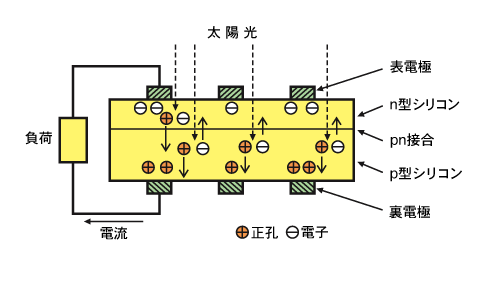
\includegraphics[width=13cm]{./fig/fig01.png}
  \caption{太陽光発電の原理}
\end{figure}

\subsection{種類}
太陽光発電の種類は,使用している材料によって細かく分けられているが,大別すると図.2のようになる.\\
\begin{figure}[H]
  \centering
  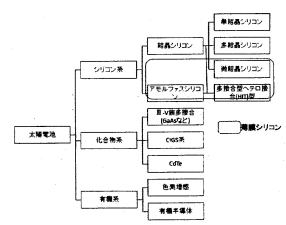
\includegraphics[height=7cm]{./fig/fig02.png}
  \caption{太陽光発電の種類}
\end{figure}

\section{実験装置回路}
\begin{figure}[H]
  \centering
  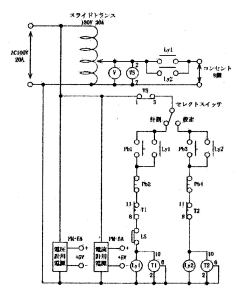
\includegraphics[height=7cm]{./fig/fig03.png}
  \caption{実験装置回路}
\end{figure}

\section{使用機器}
太陽電池実験装置:KENTAC6510\\
ライト:株式会社シバタ,110V 50/6Hz 200W\\
照度計:CUSTOM LX-1332D,DIGITAL LIGHT METER\\

\section{実験方法}
測定上の注意\\
 実験装置のセレクトスイッチは以下の特性を持っているので,測定の際はすばやく読み取ること.\\
 設定:太陽電池がセットされていなくても,「ON」にしたときランプが約 30 秒点灯する. \\
 測定:太陽電池がセットされている場合に限り,約5秒点灯する.\\

\subsection{開放電圧の照度依存性試験}
\begin{enumerate}
  \item 実験装置のコンセントを差し込む前に以下の設定を行う.\\
  ・負荷スイッチは「OFF」にする.\\
  ・ スライドトランスは「0」にする.
  \item 照度計を太陽電池脇のほぼ中心にセットする.以降,照度計は極力動かさないこと.
  \item セレクトスイッチを設定にセット,装置の照明を ON にすることで,照度の設定ができる.100lx が理想だが,実験室の原明を感知するときがあるので,その時は最低値に設定する.
  \item セレクトスイッチを測定にセット,装置の照明を ON にすることで,各数値を読むことができる.この項目では発生電圧を読み取る.
  \item 照度を対数的に上げていき同様の測定を行う(最高照度は 20000lx).
\end{enumerate}

\subsection{短絡電流の照度依存性試験}
\begin{enumerate}
  \item 以下の設定を行う.\\
  ・ 負荷スイッチは「ON」にする.\\
  ・負荷抵抗は「100\%」にする.\\
  ・ スライドトランスは「0」にする.
  \item 照度の設定は,5.1 と同様に行い,発電電流を読み取る.
\end{enumerate}

\subsection{電圧電流特性の照度依存性試験}
\begin{enumerate}
  \item 以下の設定を行う.\\
  ・ 負荷スイッチは「ON」にする.\\
  ・ 負荷抵抗は「0\%」にする.\\
  ・スライドトランスは「0」にする.
  \item 照度の設定は,5.1 を参照.
  \item 一定限度のもと,負荷抵抗を 0\% から 100\%まで増加し,それぞれの発電電圧および発電電流を読み取る.
\end{enumerate}

\newpage
\section{結果}
\subsection{開放電圧の照度依存性試験}
 測定結果を表1に示す.また,グラフを短絡電流の照度依存特性と共に図4に示す.\\

\begin{table}[H]
  \small
  \centering
  \caption{開放電圧の照度依存特性}
  \begin{tabular}{rrr}
\toprule
\multicolumn{1}{c}{照度(目標値)[lx]} & \multicolumn{1}{c}{照度(実測値)[lx]} & \multicolumn{1}{l}{発生電圧[V]} \\
\midrule
100   & 100.8 & 11.0 \\
200   & 201   & 13.7 \\
300   & 304   & 14.7 \\
400   & 402   & 15.4 \\
500   & 503   & 15.8 \\
600   & 598   & 16.1 \\
700   & 711   & 16.4 \\
800   & 798   & 16.6 \\
900   & 896   & 16.7 \\
1000  & 1050  & 16.9 \\
2000  & 2100  & 17.9 \\
3000  & 2990  & 18.2 \\
4000  & 3970  & 18.5 \\
5000  & 5050  & 18.7 \\
6000  & 5970  & 18.8 \\
7000  & 6970  & 18.9 \\
8000  & 7960  & 19.0 \\
9000  & 9060  & 19.1 \\
10000 & 10700 & 19.1 \\
20000 & 20500 & 19.5 \\
最大値   & 25500 & 19.6 \\
\bottomrule
\end{tabular}

\end{table}

\newpage
\subsection{短絡電流の照度依存性試験}
 測定結果を表2に示す.また,グラフを開放電圧の照度依存特性と共に図4に示す.\\
\begin{table}[H]
  \small
  \centering
  \small
  \caption{短絡電流の照度依存特性}
  \begin{tabular}{rrrrrrr}
\toprule
\multicolumn{1}{l}{電流I[A]} & \multicolumn{1}{l}{平均[mWb]} & \multicolumn{1}{l}{磁束Φ[Wb]} & \multicolumn{1}{l}{磁界H[A/m]} & \multicolumn{1}{l}{磁束密度B[T]} & \multicolumn{1}{l}{透磁率μe[H/m]} & \multicolumn{1}{l}{比透磁率μs} \\
\midrule
0.05  & 7.96  & 0.0003183 & 25.00 & 0.531 & 0.02122 & 16886.34 \\
0.10  & 10.18 & 0.0004073 & 50.00 & 0.679 & 0.01358 & 10802.91 \\
0.15  & 10.52 & 0.0004208 & 75.00 & 0.701 & 0.00935 & 7441.73 \\
0.20  & 10.50 & 0.0004200 & 100.00 & 0.700 & 0.00700 & 5570.69 \\
0.30  & 14.20 & 0.0005679 & 150.00 & 0.947 & 0.00631 & 5021.69 \\
0.40  & 16.57 & 0.0006627 & 200.00 & 1.105 & 0.00552 & 4394.93 \\
0.50  & 16.66 & 0.0006665 & 250.00 & 1.111 & 0.00444 & 3536.10 \\
0.60  & 18.74 & 0.0007497 & 300.00 & 1.249 & 0.00416 & 3314.25 \\
\bottomrule
\end{tabular}
\end{table}

\begin{figure}[H]
  \centering
  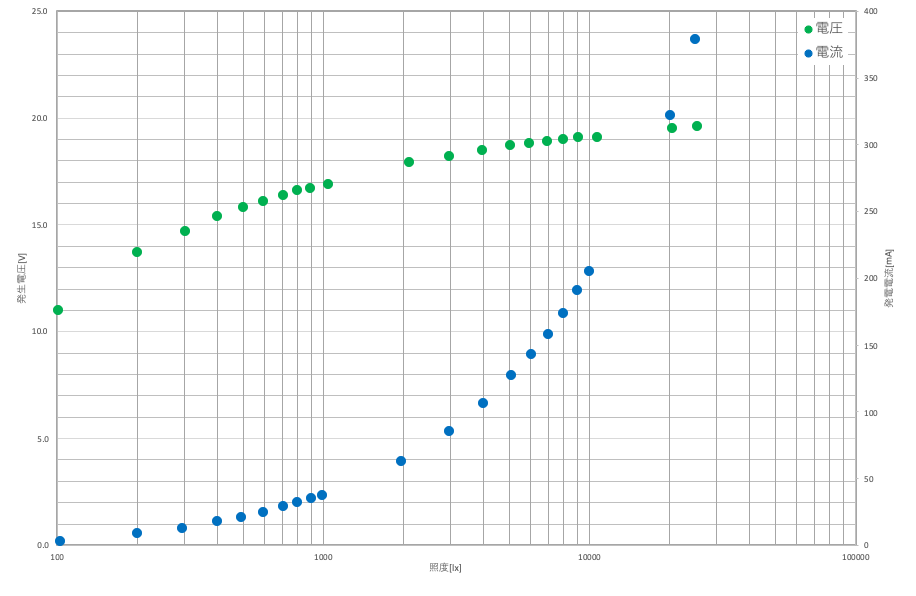
\includegraphics[width=14.3cm]{./fig/fig04.png}
  \caption{開放電圧及び短絡電流の照度依存特性}
\end{figure}

\subsection{電圧電流特性の照度依存性試験}
\begin{table}[H]
  \small
  \centering
  \caption{各発電電圧における発電電流と最大負荷電力の関係(200lx)}
  \begin{tabular}{@{}rrrr@{}}
  \toprule
  \multicolumn{1}{c}{負荷抵抗} & \multicolumn{1}{c}{発電電圧{[}V{]}} & \multicolumn{1}{c}{発電電流{[}mA{]}} & \multicolumn{1}{c}{電力{[}mW{]}} \\ \midrule
  0  & 2.3 & 8  & 18.4\\
  5  & 2.2 & 9  & 19.8\\
  10 & 2.1 & 9  & 18.9\\
  15 & 2.0 & 8  & 16.0\\
  20 & 2.0 & 9  & 18.0\\
  25 & 1.9 & 9  & 17.1\\
  30 & 1.6 & 9  & 14.4\\
  35 & 1.5 & 9  & 13.5\\
  40 & 1.4 & 8  & 11.2\\
  45 & 1.3 & 8  & 10.4\\
  50 & 1.2 & 8  & 9.6 \\
  55 & 1.0 & 9  & 9.0 \\
  60 & 0.9 & 9  & 8.1 \\
  65 & 0.8 & 9  & 7.2 \\
  70 & 0.7 & 9  & 6.3 \\
  75 & 0.6 & 9  & 5.4 \\
  80 & 0.5 & 9  & 4.5 \\
  85 & 0.3 & 9  & 2.7 \\
  90 & 0.2 & 9  & 1.8 \\
  95 & 0.1 & 9  & 0.9 \\
  100 & 0.1 & 1 & 0.1 \\ \bottomrule
\end{tabular}
\end{table}

\begin{table}[H]
  \small
  \centering
  \caption{各発電電圧における発電電流と最大負荷電力の関係(2000lx)}
  \begin{tabular}{@{}rrrr@{}}
  \toprule
  \multicolumn{1}{c}{負荷抵抗} & \multicolumn{1}{c}{発電電圧{[}V{]}} & \multicolumn{1}{c}{発電電流{[}mA{]}} & \multicolumn{1}{c}{電力{[}mW{]}} \\ \midrule
  0   & 12.3 & 57 & 701.1\\
  5   & 12.0 & 58 & 696.0\\
  10  & 11.4 & 58 & 661.2\\
  15  & 10.7 & 59 & 631.3\\
  20  & 10.7 & 59 & 631.3\\
  25  & 9.8  & 60 & 588.0\\
  30  & 9.8  & 60 & 588.0\\
  35  & 8.3  & 61 & 506.3\\
  40  & 7.7  & 61 & 469.7\\
  45  & 7.1  & 62 & 440.2\\
  50  & 6.3  & 62 & 390.6\\
  55  & 5.6  & 62 & 347.2\\
  60  & 5.0  & 63 & 315.0\\
  65  & 4.4  & 63 & 277.2\\
  70  & 3.7  & 64 & 236.8\\
  75  & 3.0  & 64 & 192.0\\
  80  & 2.3  & 64 & 147.2\\
  85  & 1.6  & 65 & 104.0\\
  90  & 1.2  & 64 & 76.8 \\
  95  & 0.4  & 64 & 25.6 \\
  100 & 0.1  & 64 & 6.4  \\ \bottomrule
\end{tabular}
\end{table}

\begin{table}[H]
  \small
  \centering
  \caption{各発電電圧における発電電流と最大負荷電力の関係(20000lx)}
  \begin{tabular}{@{}rrrr@{}}
  \toprule
  \multicolumn{1}{c}{負荷抵抗} & \multicolumn{1}{c}{発電電圧{[}V{]}} & \multicolumn{1}{c}{発電電流{[}mA{]}} & \multicolumn{1}{c}{電力{[}mW{]}} \\ \midrule
  0   & 19.1 & 90  & 1719.0\\
  5   & 19.0 & 94  & 1786.0\\
  10  & 18.9 & 99  & 1871.1\\
  15  & 18.9 & 105 & 1984.5\\
  20  & 18.8 & 111 & 2086.8\\
  25  & 18.7 & 117 & 2187.9\\
  30  & 18.6 & 130 & 2418.0\\
  35  & 18.5 & 141 & 2608.5\\
  40  & 18.4 & 153 & 2815.2\\
  45  & 18.2 & 164 & 2984.8\\
  50  & 18.0 & 184 & 3312.0\\
  55  & 17.8 & 203 & 3613.4\\
  60  & 17.5 & 225 & 3937.5\\
  65  & 17.0 & 249 & 4233.0\\
  70  & 15.8 & 281 & 4439.8\\
  75  & 13.4 & 291 & 3899.4\\
  80  & 10.2 & 298 & 3039.6\\
  85  & 7.4  & 305 & 2257.0\\
  90  & 5.1  & 309 & 1575.9\\
  95  & 1.9  & 315 & 598.5 \\
  100 & 0.1  & 318 & 31.8\\ \bottomrule
\end{tabular}
\end{table}

\begin{figure}[H]
  \centering
  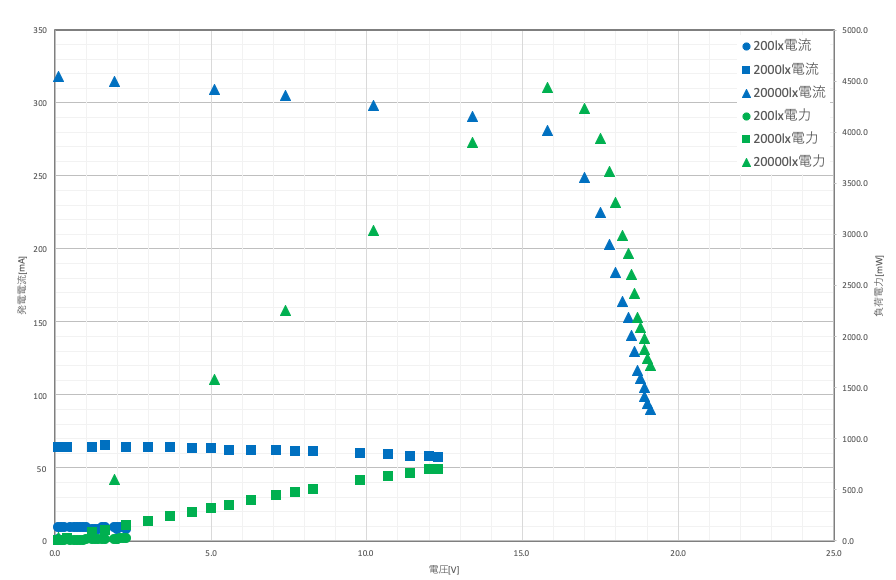
\includegraphics[width=15cm]{./fig/fig05.png}
  \caption{各発電電圧における発電電流と最大負荷電力の関係}
\end{figure}

\newpage
\section{考察}
 開放電圧の照度依存性試験では,図3の開放電圧のグラフを見ると,照度をあげるとそれに伴い発生電圧も単調に上昇していくことがわかる.しかし,増加量は一定値ではなく,照度をあげるほど増加量は低下していくことが読み取れる.今回は実験器具の関係で25500lxまでの測定で終わったが,さらに大きい照度の光を当てると,発生電圧は20.0V付近で飽和していくと考えられる.\\

 短絡電流の照度依存性試験では,図3の短絡電流のグラフを見ると,開放電圧と同様に照度をあげるとそれに伴い発生電圧も単調に上昇していくことがわかる.しかし,その増加量は一定ではなく,開放電圧とは逆に下がっていくことが確認できる.ここで,開放電圧と短絡電流をもとに各照度における最大出力を求めた.これを表6および図6に示す.このグラフから,最大出力は照度にほぼ比例することがうかがえる.このことから,照度に対する出力は比例関係であるが,開放電圧は徐々に飽和していくため,相補的に短絡電流は急激に増加していったと考える.\\

 各発電電圧における発電電流と最大負荷電力の関係について,どの照度においても電圧が増加するにつれて発生電流は低下している.ここで,20000lxでの負荷電流に着目すると,16.0V付近から急激に減少していることが確認できる.それに伴い,負荷電力も16.0V付近でピーク値4439.8mWを取っていることがわかる.このピークのポイントは最も大きな有効電力が得られる点として,最適動作点と呼ばれる.\footnote{太陽電池の出力特性と評価方法 - EKO 英弘精機株式会社,https://eko.co.jp/solar/sol\_apps/0304.html,2019-7-23閲覧}この最適動作点をすぎると急激に出力が低下するため,発電を安定させるにはこの点よりも小さい発電電圧になるように,負荷抵抗を調整する必要があると考察する.なお,200lx,2000lxでの測定では,発電電圧が最適動作点まで到達しなかった.照度2000lx以上の数点で測定を行えばそれぞれの最適動作点を比較して,より深い考察が得られたと考える.

\newpage
\begin{table}[htbp]
  \centering
  \caption{照度に対する最大出力}
  \begin{tabular}{rrrr}
  \toprule
  \multicolumn{1}{c}{照度(目標値)[lx]} & \multicolumn{1}{l}{発生電圧[V]} & \multicolumn{1}{l}{発電電流[mA]} & \multicolumn{1}{l}{最大出力[mW]} \\
  \midrule
  100   & 11.0  & 3     & 33 \\
  200   & 13.7  & 9     & 123.3 \\
  300   & 14.7  & 13    & 191.1 \\
  400   & 15.4  & 18    & 277.2 \\
  500   & 15.8  & 21    & 331.8 \\
  600   & 16.1  & 25    & 402.5 \\
  700   & 16.4  & 29    & 475.6 \\
  800   & 16.6  & 32    & 531.2 \\
  900   & 16.7  & 35    & 584.5 \\
  1000  & 16.9  & 37    & 625.3 \\
  2000  & 17.9  & 63    & 1127.7 \\
  3000  & 18.2  & 85    & 1547 \\
  4000  & 18.5  & 106   & 1961 \\
  5000  & 18.7  & 127   & 2374.9 \\
  6000  & 18.8  & 143   & 2688.4 \\
  7000  & 18.9  & 158   & 2986.2 \\
  8000  & 19.0  & 174   & 3306 \\
  9000  & 19.1  & 191   & 3648.1 \\
  10000 & 19.1  & 205   & 3915.5 \\
  20000 & 19.5  & 322   & 6279 \\
  \bottomrule
\end{tabular}
\end{table}

\begin{figure}[H]
  \centering
  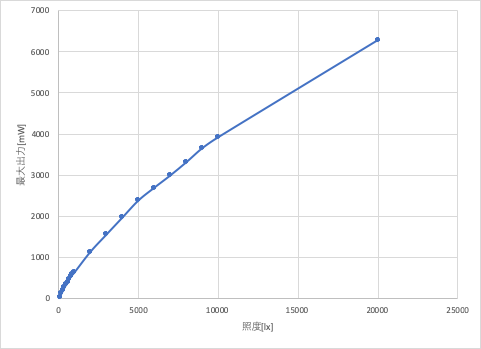
\includegraphics[width=15cm]{./fig/fig06.png}
  \caption{照度に対する最大出力}
\end{figure}

\newpage
\theendnotes

\end{document}
